\chapter{Fine-mapping Genome-wide Association Study Summary Statistics Using Functional Annotations}

\section{Introduction}\label{sec:org59556ac}


\subsection{Much of GWAS signal is non-coding}\label{sec:org3ac0b01}

Surveys of GWAS association have found that a majority of GWAS signal comes from non-coding regions of the genome.  It is believed that the majority 
of this functional variation is regulatory in nature.  Rather than modifying the function of a gene product directly, the activity of the product is modified
by modulating the abundance of the product through regulatory mechanisms: increasing or decreasing the baseline rate of transcription of DNA to RNA or degradation of mRNA back into individual nucleotides.  


\subsection{rewrite me}
This integrated analysis revealed a significant enrichment of heritability estimates for gestational duration in decidua-derived stromal cell genomic regions marked by open chromatin or histone marks. Leveraging those functional annotations in a Bayesian statistical framework, we discovered additional loci associated with gestational duration and improved fine mapping in regions associated with gestational duration. Finally, using promoter capture Hi-C (pcHi-C), we linked functionally-annotated gestational age-associated variants to their putative target genes. More generally, these functional annotations should prove a valuable resource for studying other pregnancy-related conditions, such as preeclampsia and recurrent miscarriage, as well as conditions associated with endometrial dysfunction, such as endometriosis and infertility. 

\section{Materials and Methods}\label{sec:org39326e2}

\subsection{Functional Genomic Data}\label{sec:org702e301}
  
Placentas were collected from six African American women (\(\geq 18\) years old) following spontaneous labor.
Three of the women delivered at term (\(\geq 37\) weeks), and three delievered preterm.
All were vaginal deliveries of singleton pregnancies. Within 1 hour of delivery, $5 \times 5$ cm pieces of the membranes were
sampled from a distant location of the rupture site. Pieces were placed in DMEM-HAMS F12 media containing 10\% FBS and
1\% pen/strep. Samples were kept at 4°C and processed within 24 hours of tissue collection.

Primary MSC were derived from three women who delivered at term and three who delivered preterm using cells isolated from the decidua parietalis.
To model the process of decidualization, cells were treated with medroxyprogesterone acetate (MPA)
and cAMP for 48 hours and a paired set of untreated samples was cultured in parallel for 48 hours.
To model the trophoblast invasion process, cells were treated with Trophoblast Conditioned Medium (TCM).

Three replicates of of each cell line were studied to assess experimental variability in the three conditions.
Each of the 27 samples (3 individual lines x 3 replicates x 3 conditions) were assayed to generate transcriptomes (RNA-seq).
Open chromatin (ATAC-seq) was assayed for the decidualized cells and the TCM treated samples,
and histone modification (ChIP-seq) maps for H3K27ac, H3K4me1 and H3K4me3 marks were assayed in the control and decidualized cells.
Chromatin interaction was measured using promoter capture Hi-C in cultured primary decidua-derived mesenchymal stromal/stem cells (MSCs)
and in vitro differentiated decidual stromal cells (DSCs) as well as in TCM treated cells.



% \subsection{GWAS}

% The GWAS results used in this study were an extension of previously published results. As in the previous study, we included summary results from 23andMe
% for a GWAS of gestational duration in 42,121 mothers of European ancestry who reported gestational duration of their first 8 live singleton birth.
% Meta-analyzed those data with results of GWASs of gestational during in 14,263 European mothers from six additional studies.
% To identify candidate genes that may play a role in gestational duration and PTB, we used summary data from a GWAS of gestational duration based on a meta-analysis of a 23andMe
% GWAS (N=42,121)(5) and the results from six European data sets (N=14,263). 

% Data selectionFor the GWAS, we included only singleton pregnancies with spontaneous live birth deliveries with or without premature rupture of membranes (PROM). C-sections after spontaneous onset of 12 labor were retained. Medically indicated induced deliveries or C-sections were excluded. Pregnancies with known gestational or fetal complications (e.g. placental abnormities, chorioamnionitis, preeclampsia, and congenital anomalies) and pregnancies involving pre-existing medical conditions (i.e. hypertension or diabetes) or maternal risk exposure (e.g. drug use during pregnancy) known be associated with preterm birth were also excluded.GenotypingGenotyping of these data sets was conducted on DNA extracted from blood using the various SNP arrays. Specifically: the ALSPAC genotype data were generated using the Illumina HumanHap550 quad (children) and Illumina human660W quad (mothers). The cleaned genotypecalls of 465,740 SNPs of 17,842 subjects were obtained from ALSPAC. The DNBC samples were genotyped using Human660W-Quad bead arrays from Illumina. The raw genotype intensitydata (.idat) files were obtained from dbGaP and genotype calls were performed using the CRLMM algorithm (76, 77). The samples from the MoBa dataset were genotyped using the Illumina Human660W-Quadv1A bead chip (Illumina Inc.) and the genotype calls were determined using the CRLMM algorithm. For the FIN dataset, genotyping was conducted using Affymetrix 6.0 (Affymetrix, California, United States) and various other Illumina arrays (Illumina, California, United States). For the Affymetrix SNP Array 6.0, genotype calls were determined using the CRLMM algorithm in chips that passed the vendor-suggested QC (ContrastQC > 0.4). For the Illumina chips, the genotype calling was conducted using Illumina’s genotyping module v1.94 in GenomeStudio v2011.1. The HAPO samples of European descent were genotyped using Human610-Quad array. We obtained the raw genotype intensity data (.idat) files and performed genotype calls using the CRLMM algorithm. The processed genotype calls in plink format of the GPN data set were obtained from dbGaP (phs000714.v1.p1). Data 13
% from participants of apparent duplications with others (IBD>0.8), with sex discrepancies (between known sex and genetically inferred sex), and children with high Mendelian errors (>10\%) were removed. Genotyping QCWe performed similar genotype QC across all the dataset. We first performed sample-level QC based on call rate, overall heterogeneity and sex discrepancies. We checked the pedigree relationship based on IBD analysis. Genetic ancestry was assessed by principal components analysis (PCA) anchored by 1000 Genomes reference samples. Individuals with non-European ancestry were excluded. We then performed marker level QC: SNPs with low call rate (<98\%), low minor allele frequency (<0.01) or significant deviation from Hardy-Weinberg Equilibrium (P< 5×10-6) were excluded.ImputationWe conducted genome wide imputation following a standard two-step imputation procedure: the genotype data was first pre-phased together using the Shapeit2 software (78) and then the estimated haplotypes were used to impute non-genotyped SNPs using the reference haplotypes extracted from the Phase III 1000 Genomes Project (79) using Minimac4 (80) (FIN and MoBa).Association analysisSingle-marker genetic association tests were conducted in individual data sets separately, using regression methods and imputed genotype data. Fetal sex was included as covariate. The test results from the 7 data sets were then combined by fixed effect meta-analysis using the inverse-variance method.

\subsection{Methods}\label{sec:org53944c4}


\subsubsection{Modeling Gene Expression Data}\label{sec:orgc908098}

The following sources of variation in expression data were known in addition to the primary and interaction effects: the passage number of the cell line when RNA was gathered,
the within-individual effect on gene expression, and the growth rate of the cell line.  We chose to account for the individual-level effect rather than the growth rate effect, and hoped that the estimate of the individual level effect accounts for the differences in growth rate. 

With the exception of passage number, all of the covariates of the model are
categorical. There are several ways of encoding categorical variables in a generalized linear model, and different encodings can change how the coefficient
estimates are interpreted. We here briefly describe the coding of our model, with particular emphasis on the consequence of coding on the interpretation of the coefficients.  For testing which genes are differentially expressed
between control-media treated and decidualizing-media treated cells, and similarly for testing what genes are differentially expressed between decidualizing-media treated cells and trophoblast-conditioned media cells, a standard
``treatment'' coding was used wherein decidualizing-media (\texttt{dec}) was the reference level.
One can interpret the estimates for the \texttt{ctr} and \texttt{TCM} coefficients as the change in average expression in each of those conditions relative to the \texttt{dec} condition.
The effect of term vs preterm effects were estimated using a ``sum'' coding. Instead of setting either term or preterm to be a reference level, which would carry on in our interpretation of other coefficients (i.e the \texttt{ctr} and \texttt{TCM} effects would also be interpreted as relative to either \texttt{dec}-term or \texttt{dec}-preterm), the term-preterm coefficient can be interpreted as differences in the mean expression relative to one-another.
The choice of sum coding for the term vs preterm covariate is especially important when considering how response to treatment differs between term and preterm individuals.
To formally test this hypothesis (that individuals with term births respond differently to either \texttt{dec} or \texttt{TCM} as compared to individuals with preterm births), we test for an interaction between the preterm effect
and each of the two treatment effects.  A nonzero estimate of either of these interaction terms indicates that the reponse to treatment (i.e the change in gene expression) differs between term and preterm samples.
To capture the individual level effects, instead of comparing to a particular individual, we again used a sum coding, meaning for each term and preterm,  1 covariate captures the difference between the individual 1 and individual three,and another captures the difference betweeen individual 2 and individual three.
Like passage number, individual-level effects are important to incorporate in the model, but effect-size estimates are not of direct relevance.

We used the the pseudo-alignment tool \texttt{salmon}\cite{salmon} to obtain transcript-level abundance estimates (using gencode 19 as a source of transcripts). The abundance estimates were loaded into R 
using the \texttt{tximeta} package,\cite{tximeta} which was also used to summarize the transcript-level abundance estimates into gene-level abundance estimates.  Genes with counts lower than 10 were excluded from consideration
for differential expression, as were genes for which the gene level abundance estimate was above zero in less than 5 samples.  We then used the R package \texttt{DESeq2}\cite{DESeq2} to identifiy differentially expressed genes.  For the main effect tests (i.e term vs preterm, control vs decidualized, and TCM vs decidualized)  we used the Wald test functionality for null hypothesis significance testing.  \texttt{DESeq2} includes composite null hypothesis testing functionality when using the Wald test; instead of testing against the null hypothesis  that \(\beta =  0\), one can test against the hypothesis that \(\lvert \beta \rvert \leq \theta\) where \(\theta\) is some threshold value.  Rather than adding a fold-change cutoff on top of a test against an effect size of 0,  with the composite test the FDR results remain interpretable: $p$-values and adjusted $p$-values correspond to the specific null hypothesis of interest.  This composite null-hypothesis testing was used with a log fold-change threshold of 0.2.

\subsubsection{A pipeline for fine-mapping GWAS summary statistics using functional annotations}\label{sec:org24e3fbe}

Fine mapping proceeded in three stages. In the first stage we partitioned the genome into 1,703 regions approximately independent regions using breakpoints derived from the ldetect method\cite{ldetect}.
Next, we constructed a SNP-level prior probability of causality, informed by the functional genomic datathat a particular SNP is causal.  To estimate the functionally informed SNP-level prior, We employed a Bayesian
hierarchical model TORUS\cite{torus}.  TORUS uses SNP-level annotations and GWAS summary statistics to estimate the extent to which SNPs with functional genomic annotations are likely to be causal for a trait of interest.  
TORUS takes as input GWAS summary statistics and genomic annotations, and for each annotation outputs multivariate enrichment estimates that corresponding to estimates from a logistic regression: 
the additive change in log odds for a variant being causal, conditioned on all other annotations being held constant.We ran TORUS with the gestational age GWAS summary statistics and the reproducible
H3K27ac and H3K4me1 peaks from the \texttt{dec}-treated samples, the pcHi-C contact regions, and the union of all ATAC-seq peaks to obtain enrichment estimates. A SNP-level prior was constructed from those enrichment estimates.
Lastly, fine mapping was performed using a summary statistics-based version of the “Sum of Single Effects” model (SuSiE\cite{susie}).  
In the summary statistics-based version of SuSiE, the inputs are the GWAS summary statistics in a region, the SNP-level prior for every GWAS variant, and an estimate of the LD between variants. 
As an estimate of LD, we used the unrelated European individuals from the 1000 Genomes project as a reference panel. SuSiE (as implemented in the R package “susieR”) was run on the 33 regions most 
believed to have one or more causal variants as estimated by TORUS. For each region, SuSiE was run with a uniform prior (default setting of SuSiE) and with an informed prior learned 
by TORUS. The parameter $L$ of SuSiE (maximum number of causal variants) is set at 3 when running SuSiE.  To be conservative, the pip for all SNPs in each region were multiplied by $1-\text{FDR}_{\text{TORUS}}$ to approximate the
TORUS posterior probability that the region contained at least one causal variant.

% This conservative setting ensures that the results are robust to possible LD mismatch between 
% the reference panel and the GWAS samples. In fact, when $L = 1$, the PIP of a SNP depends only on its summary statistic (effect size and standard error), prior effect size and the number of SNPs in the locus, 
% but not LD structure.  


% \subsubsection{Stratified LD score regression}\label{sec:org3173e32}

% We assessed how much of the heritability of  gestational duration is contained within ATAC-seq, H3K4me1, H3K4me3, H3K27ac and pcHi-C peaks using stratified LD score regression (S-LDSC).
% Stratified LD score regression is a generalization of LD score regression, a method for estimating the heritability of a trait using SNP-level GWAS summary statistics and SNP-level estimates
% of the amount of genetic variation tagged at each variant, known as LD scores.  Under the LD-score regression model, the expected value of the GWAS summary statistic for a variant
% (specifically 
% the expected value of the \(\chi^2\) statistic) is a linear function of the LD score at that site, and h2, the per-SNP heritability, and a an intercept parameter.  Under the S-LDSC
% model, rather than estimating a single per-SNP heritability parameter, a parameter is estimated for each of several functional annotations.  In a standard S-LDSC analysis,
% user-provided annotations are combined with a ``baseline'' set of genomicannotations from publicly available datasets.  For this analysis, stratified LD scores were calculated using
% the peaks identified as reproducible across either treated or untreated samples as annotations and the  1000 Genomes Phase 3 European individuals (Price Lab website) as a reference
% LD panel, using only the HapMap3 SNP list (also from the Price Lab website). Stratified LD regression was performed on the gestational duration GWAS using the endometrial-tissue
% derived LD scores and the “baseline” LD scores contained in version 2.2 of the LD score regression baseline LD model. We include all annotations from the baseline LD model 
% except those “flanking” annotations. This resulted in a total of 64 baseline annotations used in our S-LDSC analysis.  



\subsubsection{Gene-level summary of fine-mapping results}\label{sec:org3f48450}

To assess the enrichment of the gestational duration GWAS signal the differential expression gene signal we developed a method for summarizing our fine-mapping results at the gene level.  SNP-level PIPs were summarized as gene-level
PIPs based on one of several SNP to gene associations, and accounting for uncertainty in which gene the SNP targets.  SNPs in the \(5'\) UTR (or 2kb upstream of the \(5'\) UTR), \(3'\) UTR, or exon for a gene were assigned to that gene
, and the entire PIP for that variant is added to the total for that gene. A SNP that is within a promoter-capture HiC contact, (as called by CHiCAGO \cite{chicago}) is assigned the gene corresponding to the promoter of the
promoter-target pair.  The entire PIP for the variant is assigned to the total for the gene, unless the variant is in HiC contact with multiple promoters, in which case the PIP is split equally between the multiple genes.
If the target, i.e the non-promoter region in the promoter-capture HiC contact, lies within the gene body (the \(5'\) UTR, the \(3'\) UTR, or an exon) of a gene, that SNP is assigned to both the gene containing the variant
as well as the gene corresponding to the promoter of the promoter-capture HiC contact, and the PIP for that variant is split equally between the gene-level totals for both genes.
For variants that lay outside genes or HiC contacts, the a portion of the PIP for that variant was assigned to each gene within the fine-mapping region, with the proportion decaying exponentially with distance to the gene according
to the following function
$$\rho_{i,g}\frac{e^{\frac{-d_{i,g}}{100000}}}{\sum_{j=1}^G e^{\frac{-d_{i,j}}{100000}}}$$, with $d_{i,g}$ being the minimum distance between variant $i$ and any of gene $g$'s exons, \(5'\) UTR or \(3'\) UTR.  

We take the simplifying assumption that causal variants act through exactly one (annotated) gene. We use the following equation for the gene-level PIP:

$$\text{P}_{g} = \sum_{i \in H_g}  \frac{p_i}{h_i} + \sum_{j \in B_g} p_j + \sum_{k \not\in H_g \cup B_g} \rho_{k,g}p_k$$

In the above equation $H_g$ is the set of variants in HiC contact with gene $g$, $h_i$ is the number of HiC contacts in contact with variant $i$, $B_g$ is the set of variants within the \(5'\) UTR, the \(3'\) UTR, or an exon of gene $g$, and $H_g \cup B_g$ is the union of $H_g$ and $B_g$.

\section{Results}\label{sec:orgb8d6bf0}

\subsection{Enrichment for Gestational Duration GWAS signal in Decidual Derived Functional Annotations}

\begin{figure}
  \centering
  \begin{subfigure}[t]{\textwidth}
    \centering
    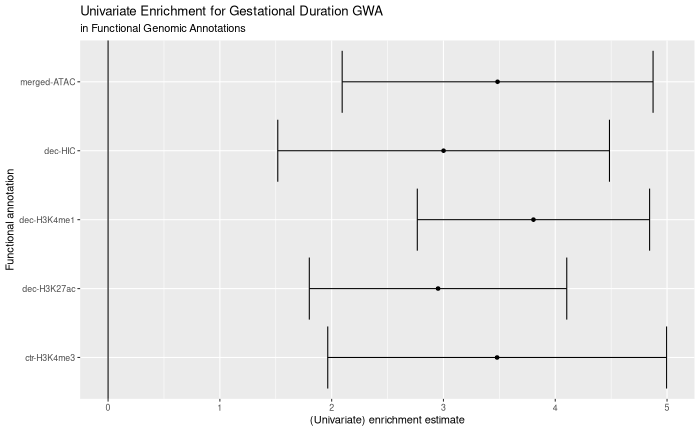
\includegraphics[width=\linewidth]{img/ptb_univ_assoc.png}
    \caption{Univariate enrichment for gestational duration GWAS signal in regulatory maps of decidua-derived stromal cells. TORUS was run on each }\label{fig:univ_assoc}
  \end{subfigure}
    \begin{subfigure}[t]{\textwidth}
    \centering
    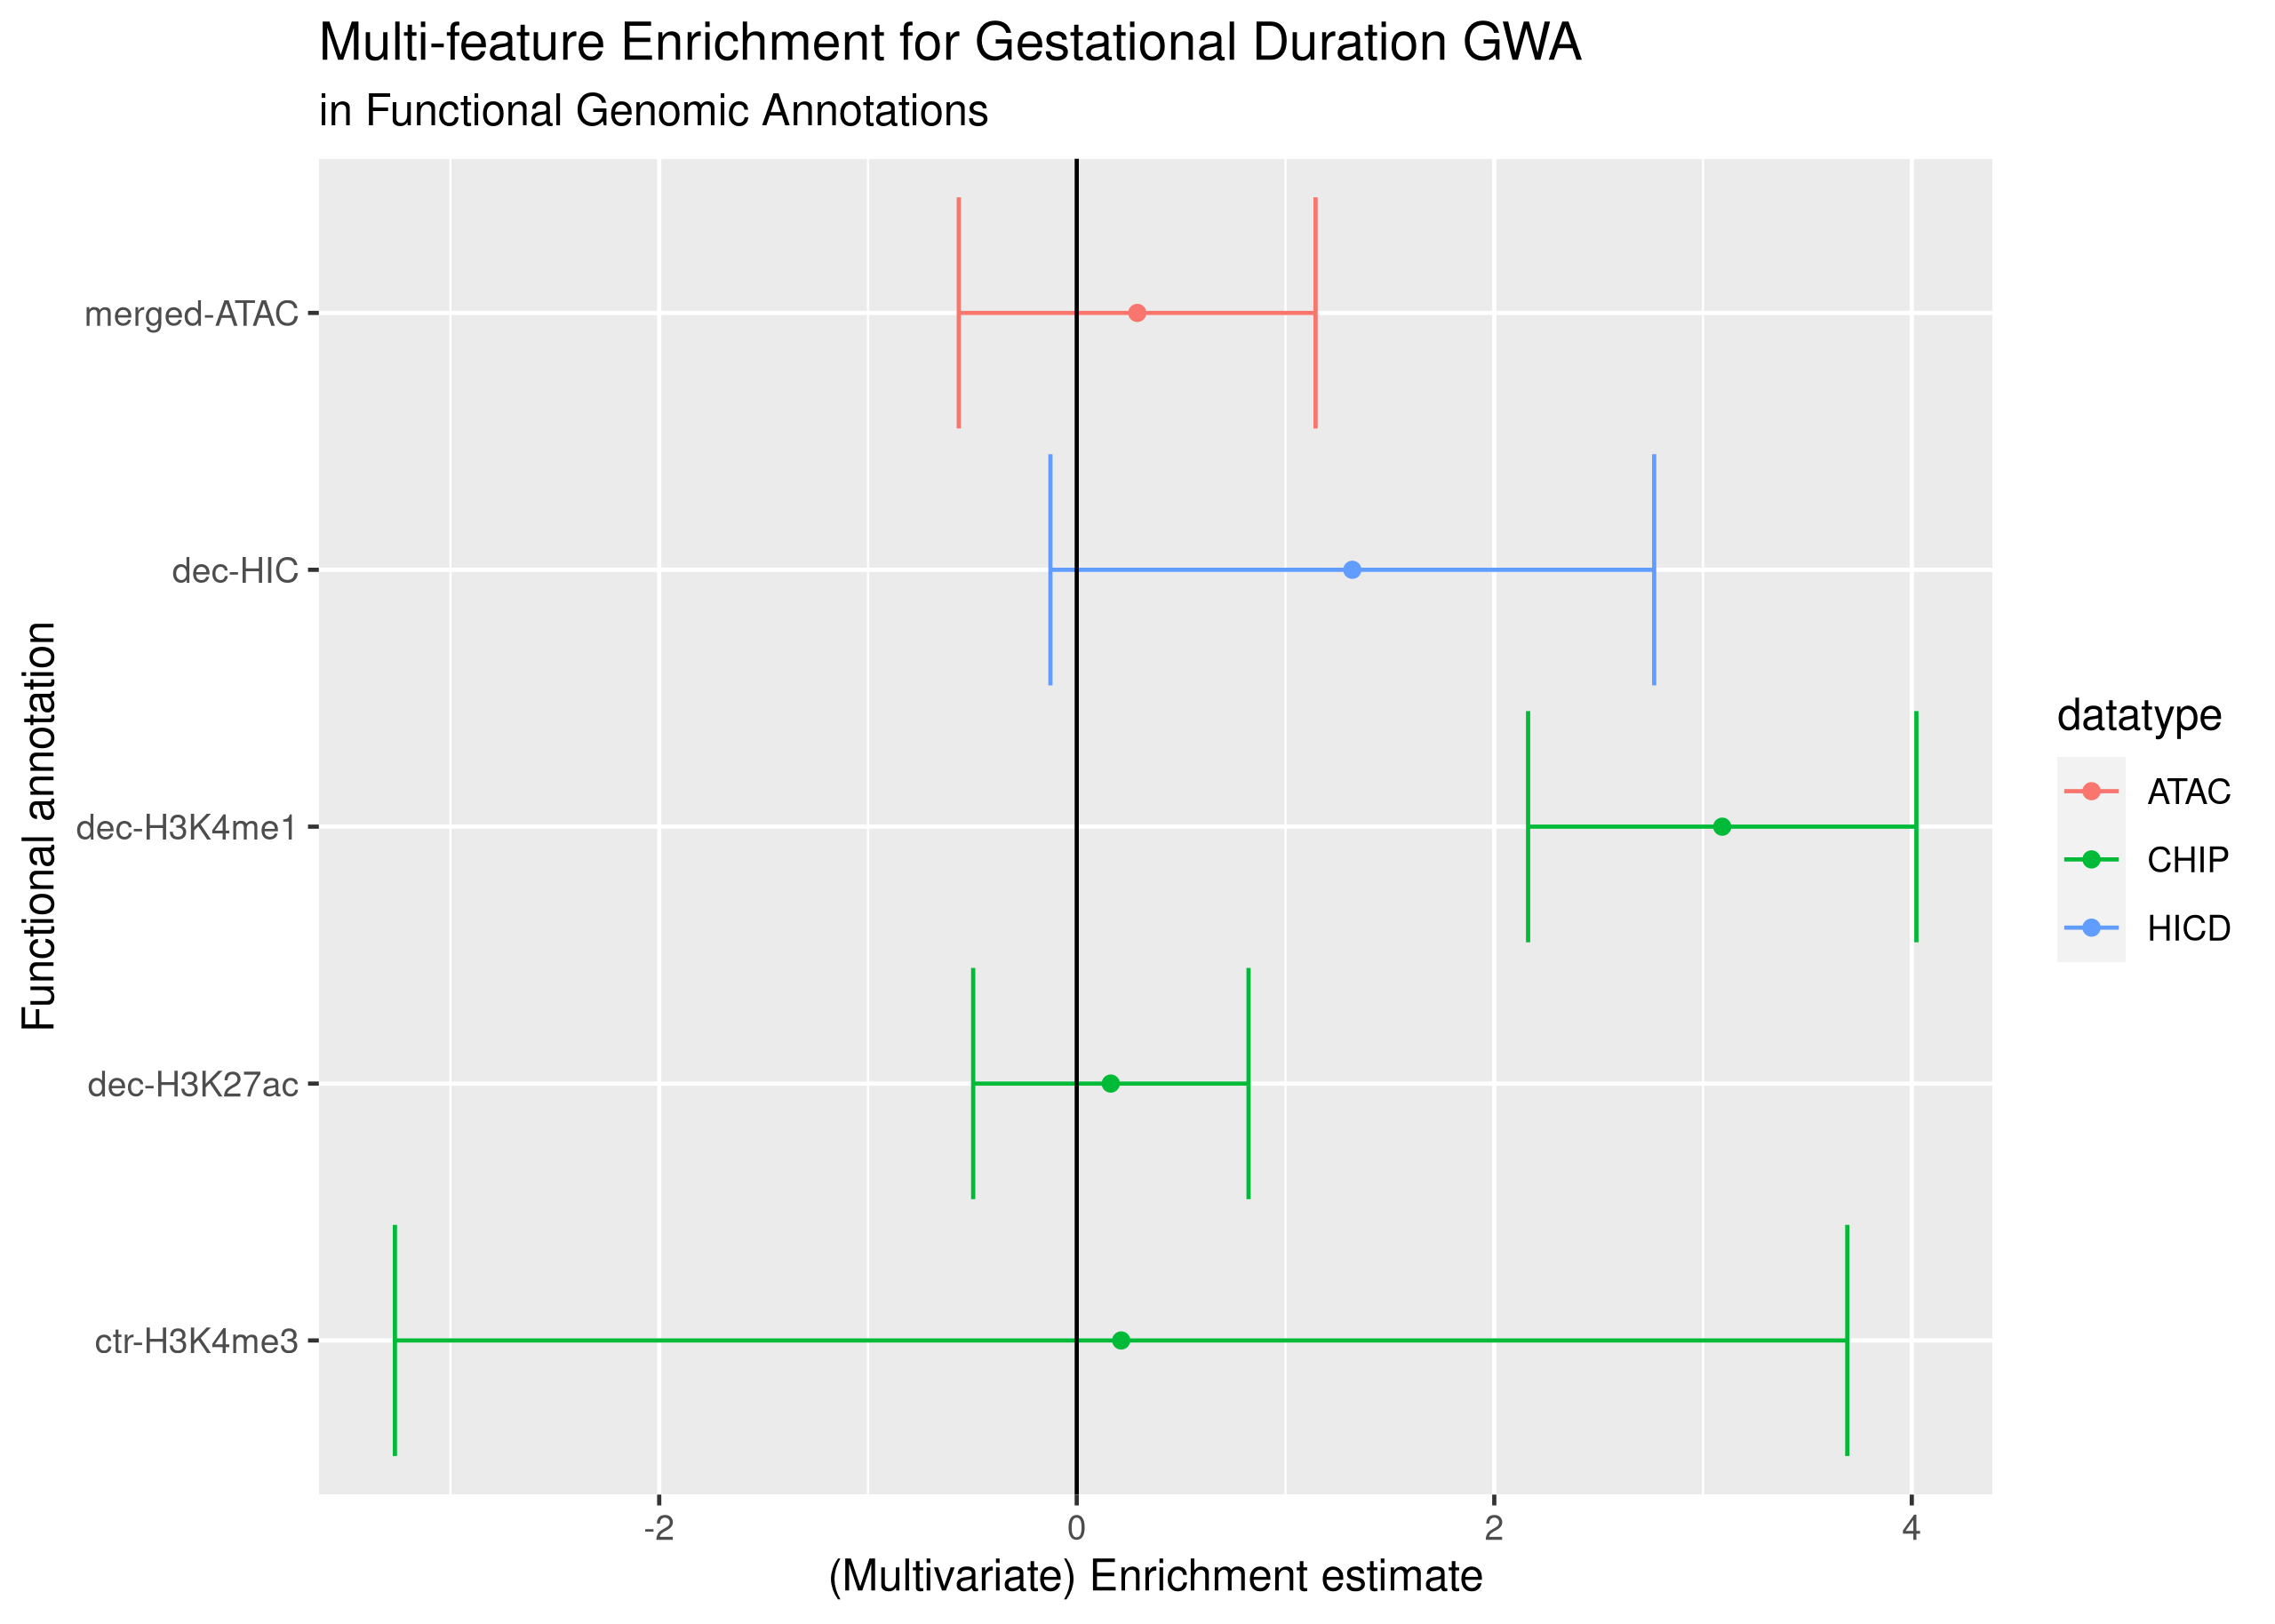
\includegraphics[width=\linewidth]{img/ptb_multiv_assoc.png}
    \caption{Multivariate enrichment for gestational duration GWAS signal}\label{fig:multiv_assoc}
    \end{subfigure}
\end{figure}



\subsection{Functionally informed gene-level fine mapping of gestational duration genes}

We developed a computational procedure to integrate the decidua stromal cell functional maps with genetic map of reproductive traits.
We posited that integrating functional maps in these pregnancy-relevant cells and leveraging statistical methods to fine-map associations
would result in 1) identifying candidate causal variants in each associated locus, 2) linking those variants to their target genes, and
3) discovering additional loci and genes associated with gestational duration. 

We first leveraged the enrichments of DSC annotations to create Bayesian prior probabilities for a variant being causal. Using prior probabilities informed by functional annotations of SNPs could increase the accuracy of fine-mapping, as shown in recent studies (8, 41). We chose H3K27ac, H3K4me1, and pcHi-C interactions from the decidualized cells, and H3K4me3 from untreated cells, and ATAC-seq peaks from any of the cells as functional genomic annotations to create informative priors using TORUS\cite{torus}. To assign a prior to each SNP, TORUS uses genome-wide summary statistics of GWAS and the functional annotations to assess how informative each annotation is in predicting causal variants. SNPs associated with functional annotations are generally assigned higher prior probabilities. Additionally, TORUS computes statistical evidence at the level of genomic blocks, defined as the probability that a block (determined by LD) contains at least one causal SNP. Without including any histone marks or chromatin accessibility annotations, TORUS implicated six autosomal blocks in the genome at FDR < 0.05, including five of the six genome-wide significant autosomal loci identified in the GWAS (p < 5x10-8).
% One locus on chromosome 3 had an FDR = 0.11, and was therefore not identified by TORUS and one locus on chromosome 9 that was not identified in the GWAS was implicated by TORUS (Supplementary File S4).
By including the functional genomic annotations from endometrial stromal cells, the number of high confidence blocks increased to ten, including all six that were significant in the gestational duration GWAS and four that were not significant in the GWAS (Supplementary File S4).  

We next performed computational fine mapping on the top these ten blocks, with the informative priors learned by TORUS, using SuSiE(43). Conceptually, SuSiE is a Bayesian version of the stepwise regression analysis commonly used in GWAS (i.e. conditioning on one variant, and testing if there is any remaining signal in a region). SuSiE accounts for the uncertainty of causal variants in each step, and reports the results in the form of posterior including probabilities (PIPs). The PIP of a variant ranges from 0 to 1, with 1 indicating full confidence that the SNP is a causal variant. If a region contains a single causal variant, the PIPs of all SNPs in the region should approximately sum to 1.  

Including the priors defined by TORUS using DSC functional annotations significantly improved fine-mapping (Figure 5A, Supplementary Table S3 and Supplementary File S5. For example, only one SNP reached PIP > 0.3 across all 10 blocks using the default setting under SuSiE (uniform prior, treating all SNPs in a block equally). This reflects the general uncertainty of pinpointing causal variants due to LD: e.g., a strong GWAS SNP in close LD with 9 other SNPs would have PIP about 0.1. By using the annotation-informed priors, 8 SNPs in six different blocks reached PIP > 0.3 (Figure 5A). In some blocks, we were able to fine-map a single high-confidence SNP, e.g. the FOXL2 locus on chromosome 3, while in other blocks, we had considerable uncertainty of the causal variants, as shown by large credible sets, i.e. the minimum set of SNPs to include the causal SNP with 95\% probability (Figure 5B). Table 1 summarizes the most probable causal variants in eight blocks (fine-mapping in the remaining two blocks produced large credible sets with no high-PIP SNPs) as well as their likely target genes based on promoter assignment or chromatin interactions from pcHi-C. We note that our results of the WNT4 locus identified rs3820282 as the likely causal variant. This is consistent with our previous results demonstrating experimentally that the T allele of this SNP disrupts the binding of estrogen receptor 1 (ESR1)(5). This SNP was among the 3 most likely SNPs in our fine-mapping study, with a PIP of 0.27 (Table 1). 



We highlight the results from two regions. In the first, two adjacent SNPs (311 bp apart), rs13141656 and rs7663453, on chromosome 4q34 did not reach genome-wide significance in the GWAS (p = 3.9 ×10-7 and 4.5 ×10-7, respectively). After using functional annotations in decidua-derived stromal cells, the block containing these SNPs was highly significant (TORUS q-value = 0.02), suggesting the presence of at least one causal variant in this block. The two SNPs together explained most of the PIP signal in the block (PIP 0.38 and 0.33, respectively, Table 1). The two SNPs are located in a region of open chromatin in endometrial stromal cells, with enhancer activity marked by both H3K27ac and H3K4me1 (Figure 5C). Only 9 of the 129 tissues from the Epigenome Roadmap(11) also had H3K27ac, H3K4me1 or H3K4me3 peaks spanning the rs13141656 locus and only 2 spanning the rs7663453 locus. In addition, this putative enhancer is bound by multiple transcription factors, including GATA2, FOXO1, NR2F2 and PGR, based on ChIP-seq data. The only physical interaction of this enhancer in the pcHi-C data in decidualized stromal cells is with the promoter of the HAND2 gene, located 277 kb away (Figure 5C). Summing over the PIPs of all SNPs whose nearby sequences interact with HAND2 via chromatin looping gives an even higher probability, 0.89, suggesting that HAND2 is very likely to be the causal gene in this region (Supplementary Table S4). HAND2 is an important transcription factor that mediates the effect of progesterone on uterine epithelium(45). Thus, in this example we identified a novel locus, the likely causal variant(s), the enhancers they act on, and an outstanding candidate gene for gestational duration and PTB.  

The second example focuses on the locus showing a strong GWAS association with gestational duration on chromosome 3q21. The lead SNP, rs144609957 (GWAS p = 4 ×10-13), is located upstream of the EEFSEC (Eukaryotic Elongation factor, Selenocysteine-TRNA Specific) gene. There is considerable uncertainty of the causal variants in this region, with 50 SNPs in the credible set and the lead SNP explaining only a small fraction of signal (PIP = 0.02). Among all 12 SNPs with PIP > 0.01, 11 have functional annotations, most commonly H3K4me1 and pcHi-C interactions. Interestingly, for nine SNPs (first 3 shown in Table 1), the sequences in which they are located physically interact with the promoter of GATA2 in the pcHi-C data, but not with any other promoters in the region (Supplementary Figure S3). The PIPs of all SNPs in the genomic regions that likely target GATA2 through chromatin looping sum to 0.68 (Supplementary Table S5). Thus, despite uncertainty of causal variants in this region, our results implicate GATA2 as a candidate causal gene in endometrial stromal cells. GATA2 is a master regulator of embryonic development and differentiation of tissue-forming stem cells(46). As support for the possible role of GATA2 in pregnancy, GATA2 deficient mice show defects in embryo implantation and endometrial decidualization(34), making this another excellent candidate causal gene for gestational duration and PTB. 


\begin{figure}
  \centering
    \begin{subfigure}[t]{\textwidth}
    \centering
    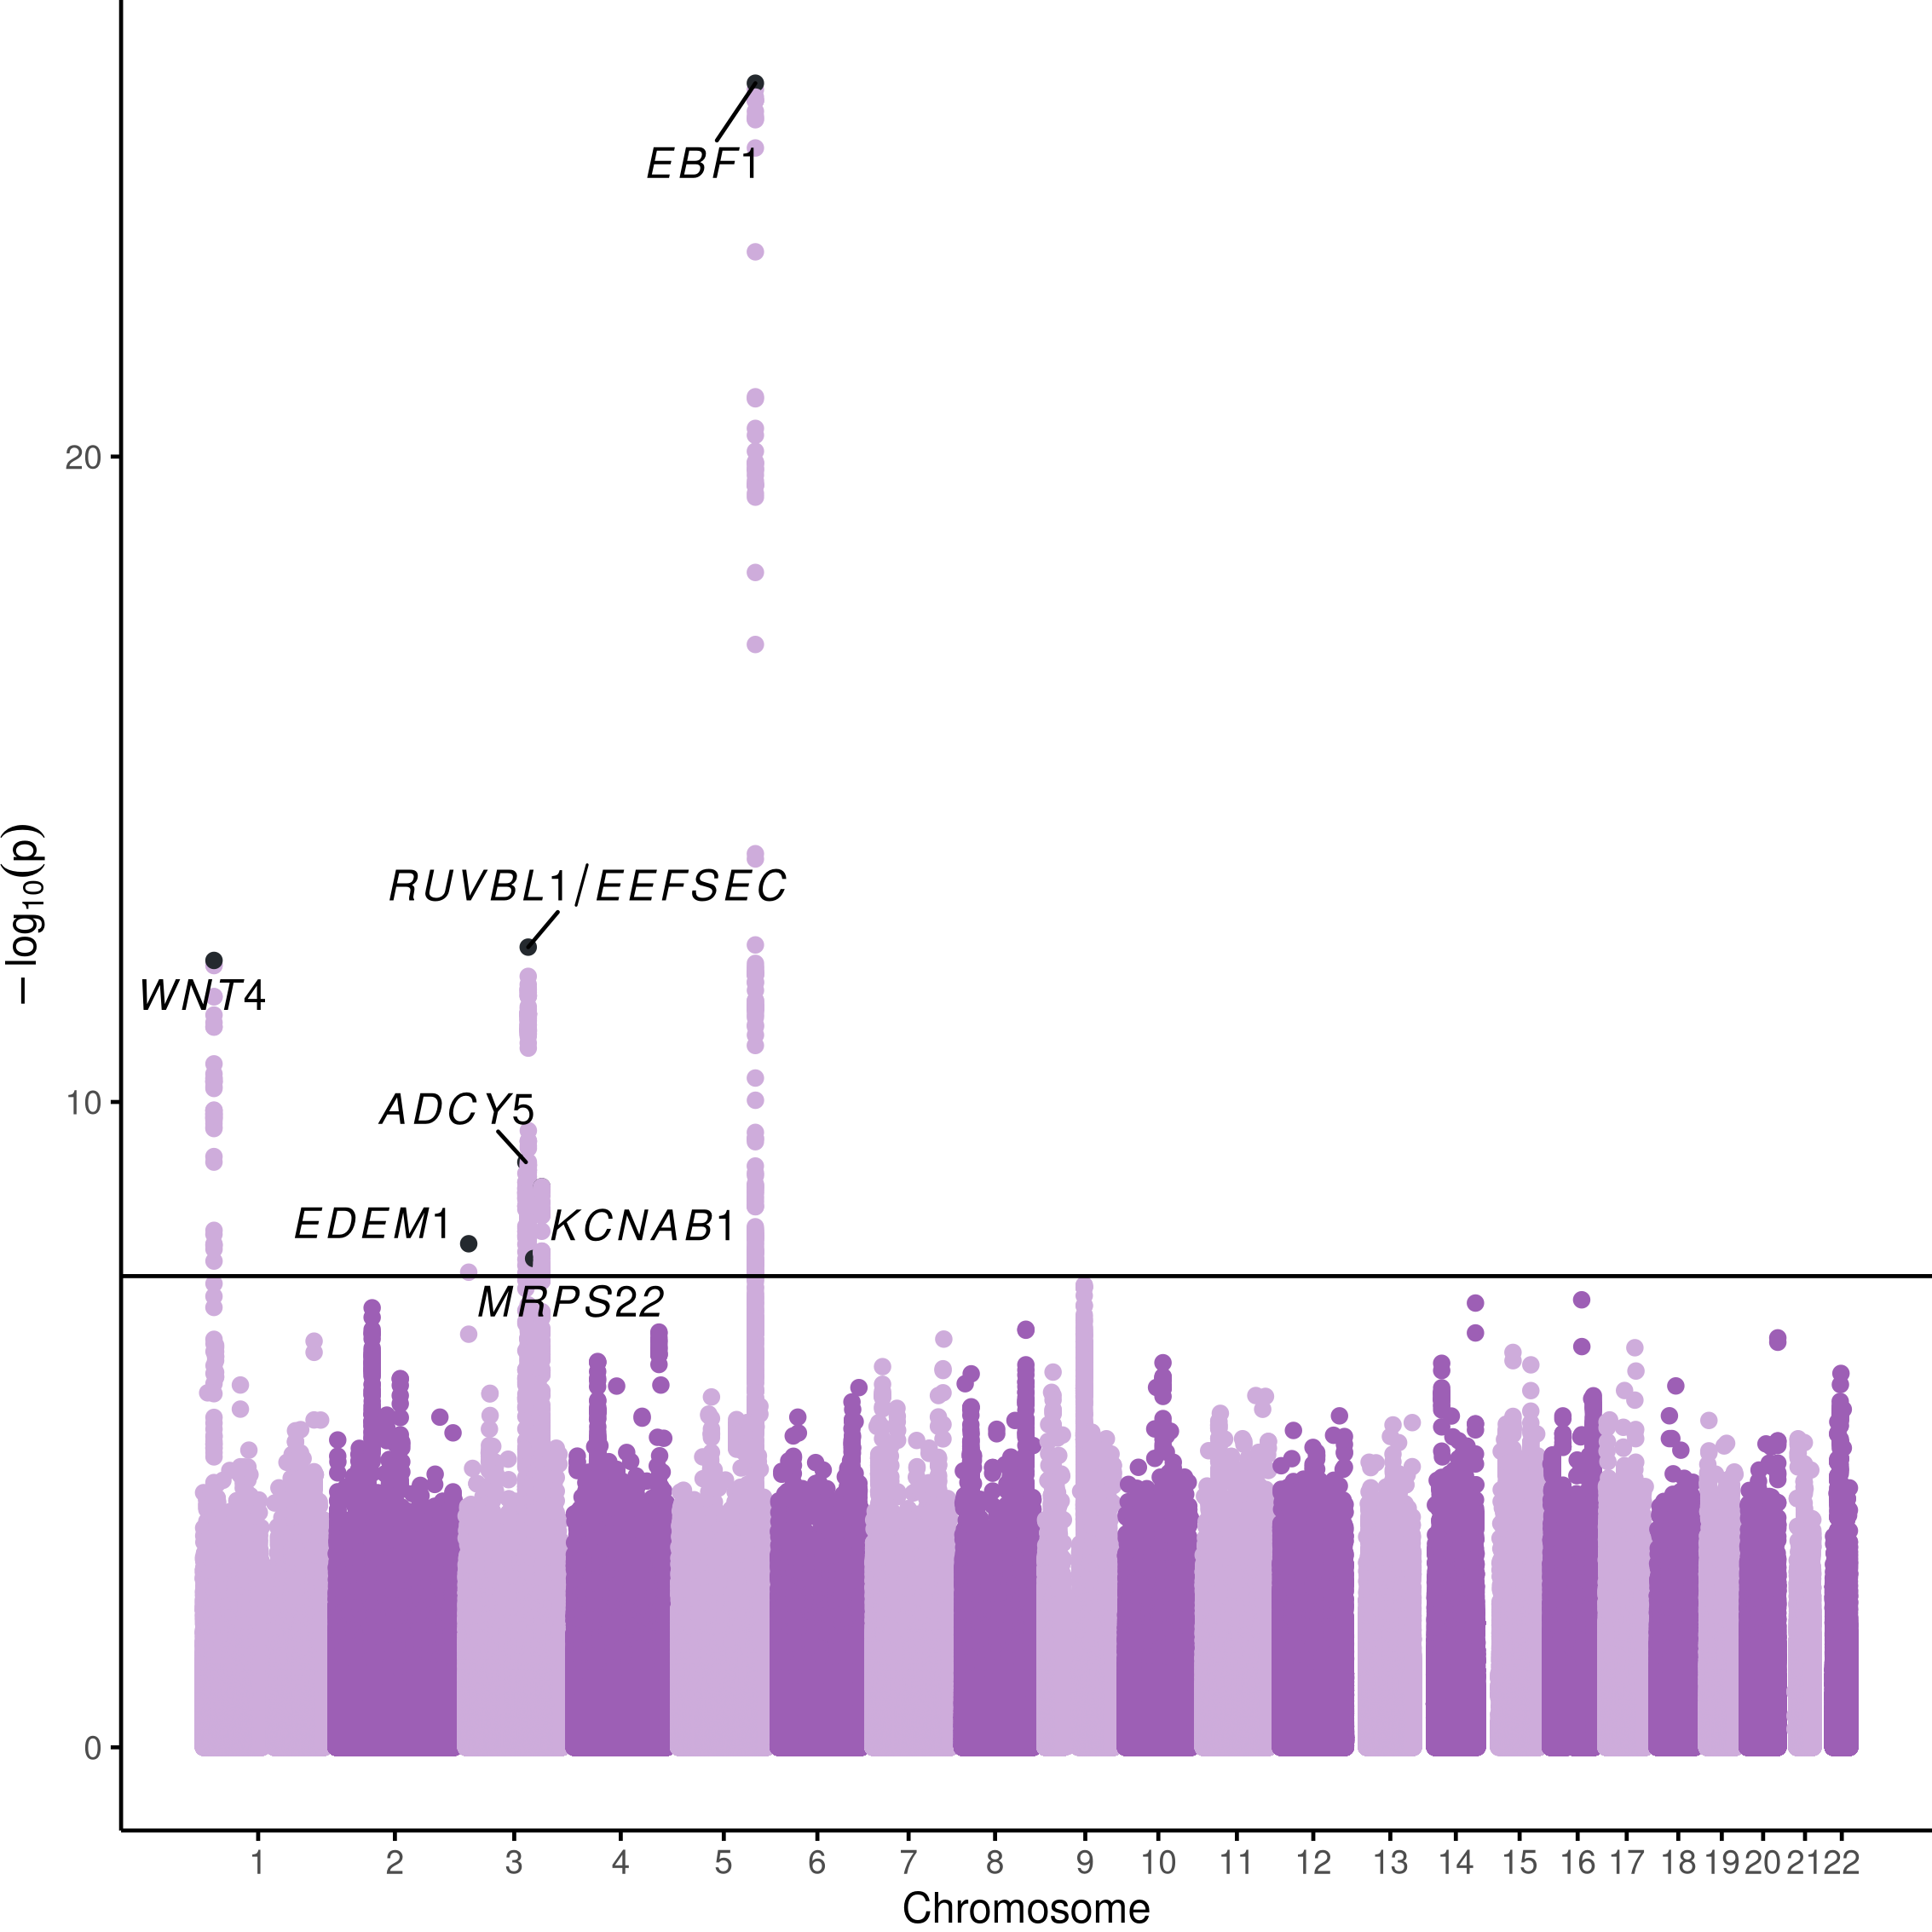
\includegraphics[width=\linewidth]{img/FigureS_Manhattan_plot.png}
    \caption{Manhattan plot of a GWAS for gestational duration GWAS. The horizontal black line denotes the threshold for genome-wide significance ($p < 5 \times 10^{-8}$). For the 6 independent genome-wide significant loci, the most significant p-value is highlighted in black, and labeled with the nearest gene(s).}\label{fig:manhattan}
  \end{subfigure}
\end{figure}

\begin{figure}
  \centering
  \begin{subfigure}[t]{\textwidth}
    \centering
    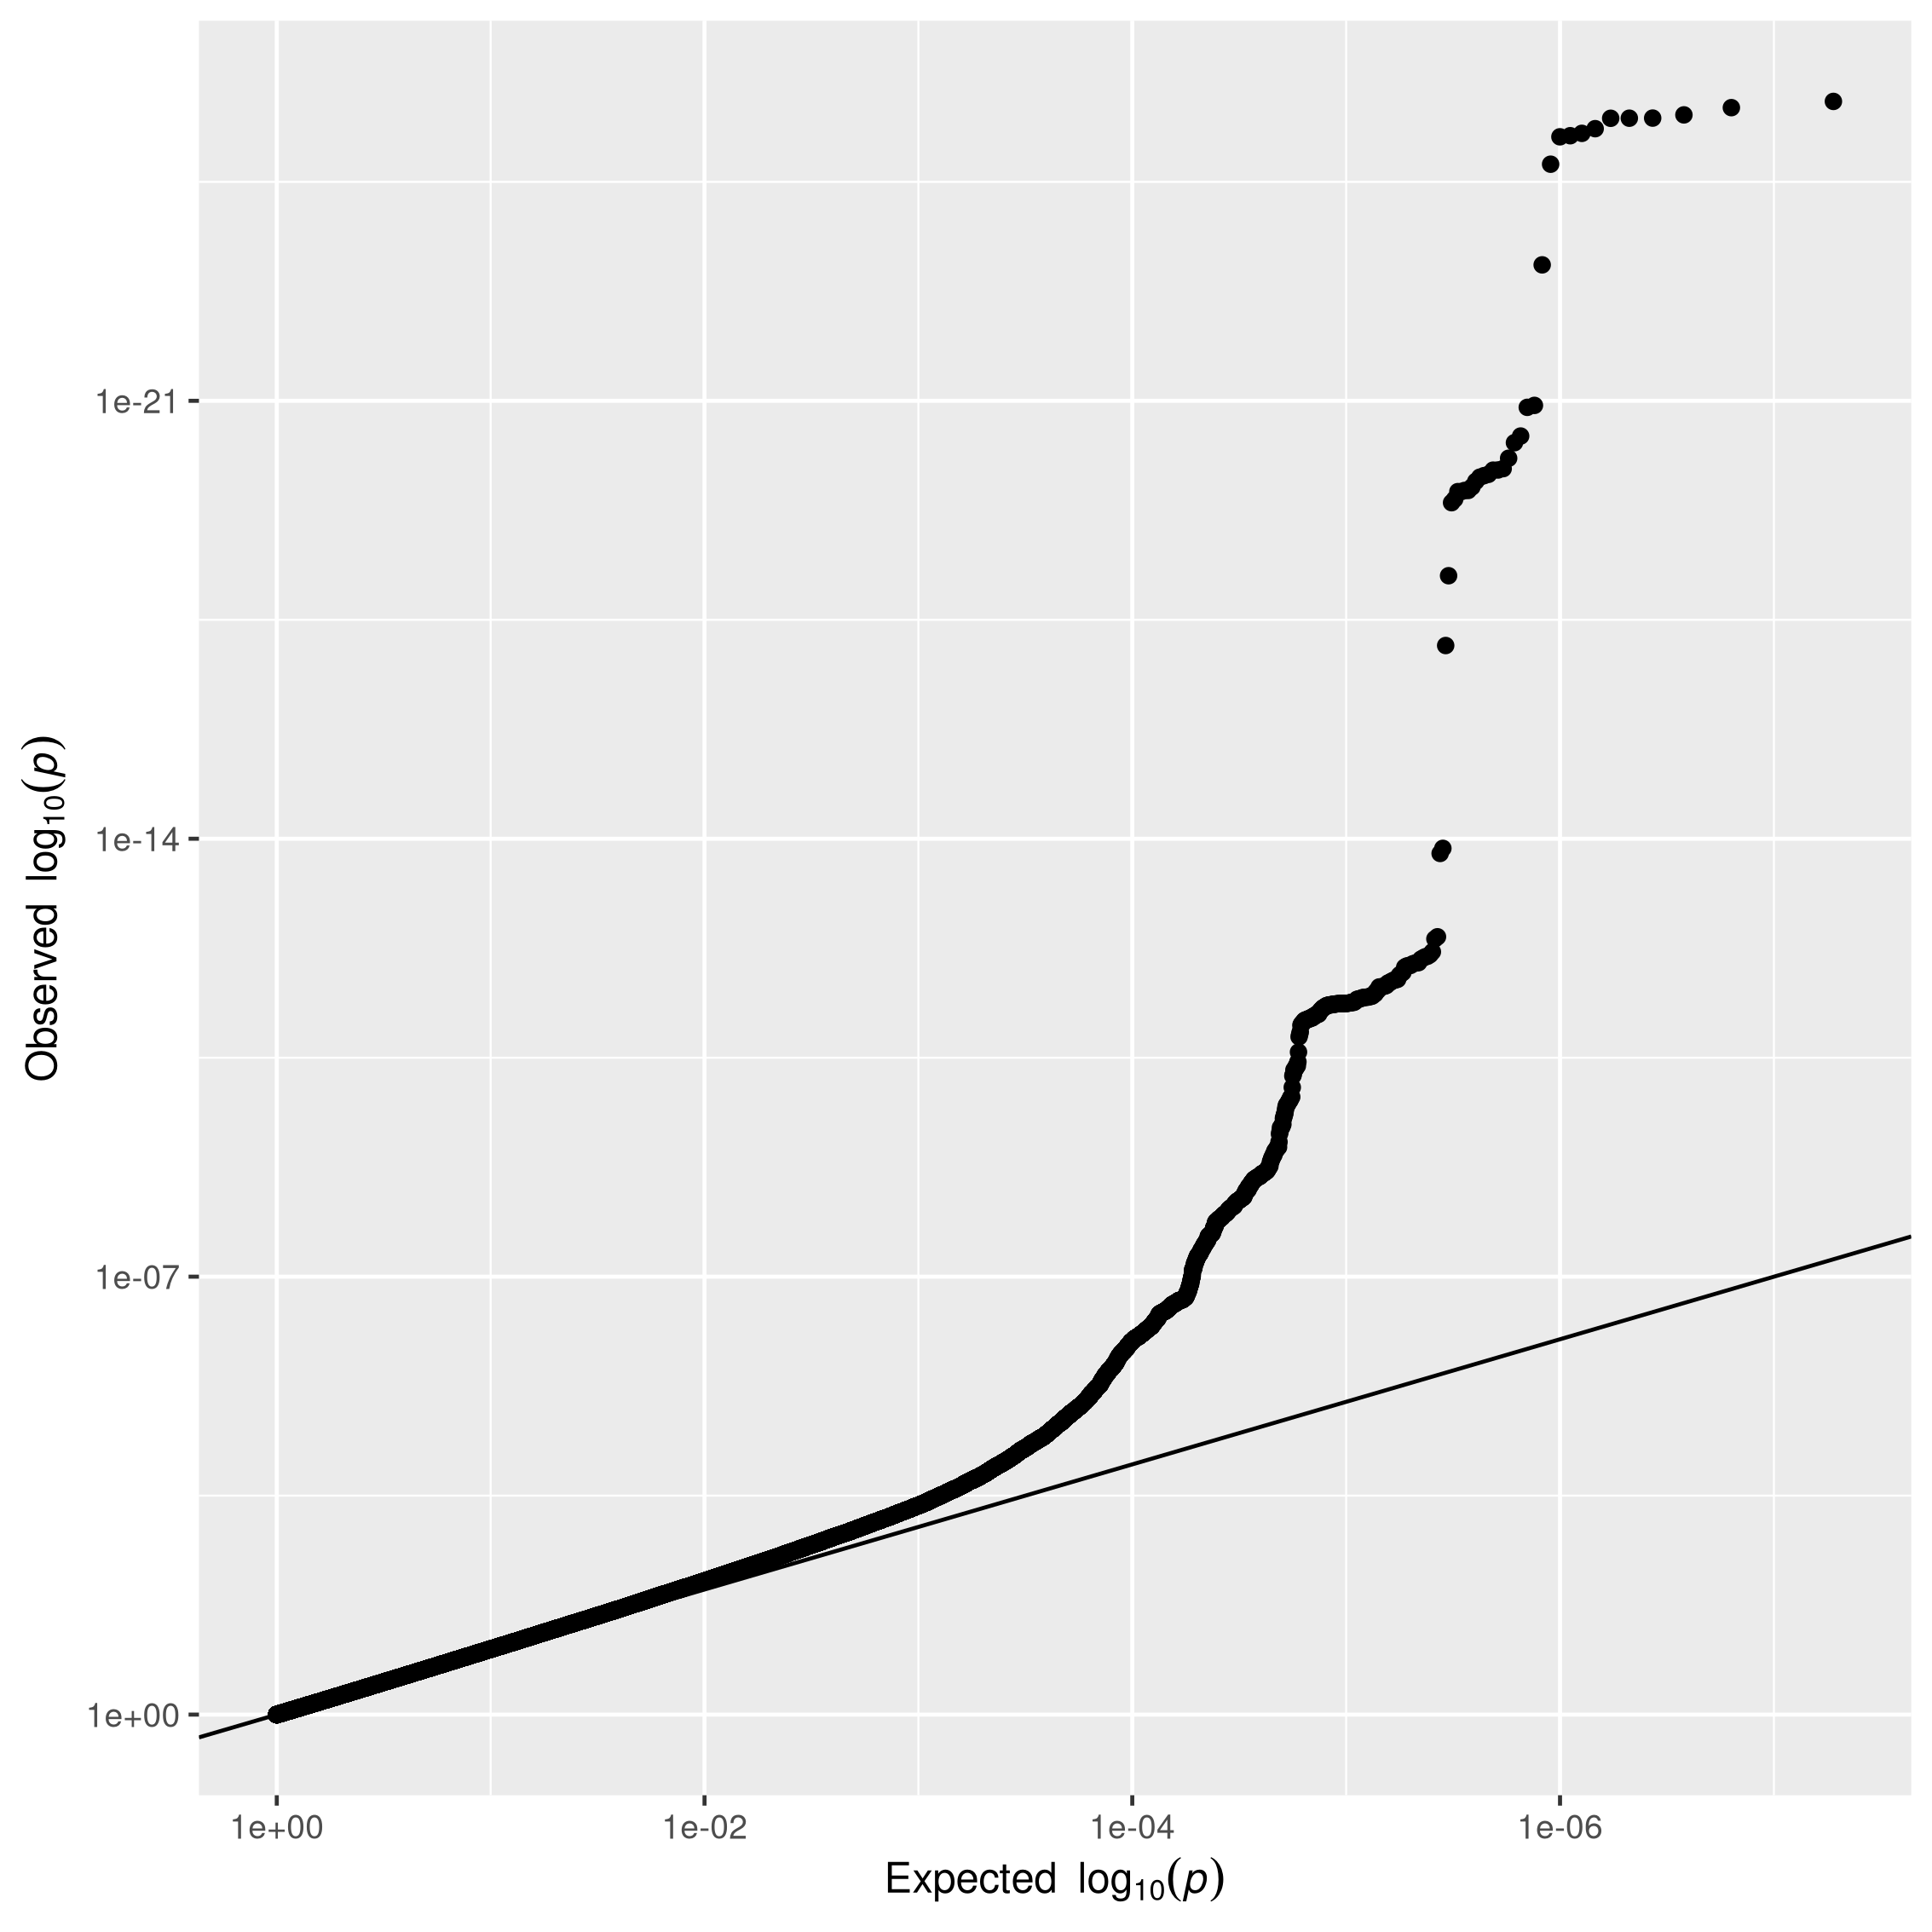
\includegraphics[width=\linewidth]{img/FigureS_qq_plot.png}
    \caption{QQ plot of p-values from the GWAS of gestational duration.}\label{fig:qqplot}
  \end{subfigure}
\end{figure}


\begin{figure}
  \centering
  \begin{subfigure}[t]{\textwidth}
    \centering
    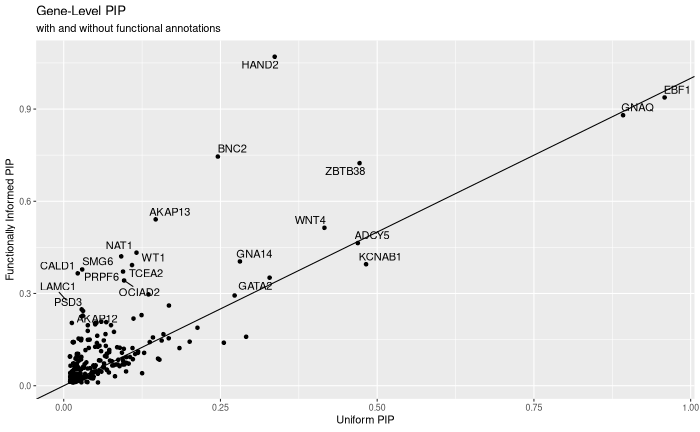
\includegraphics[width=\linewidth]{img/null-gene-gene-comp.png}
    \caption{Gene-level PIPs under the functionally informed model as compared to the uniform model.  The same variant-gene assignment was used for both models.  Genes above the black diagonal line have a higher gene-level PIP under the functionally-informed model compared to the uniform model.  }\label{fig:univ_assoc}
  \end{subfigure}
    \begin{subfigure}[t]{\textwidth}
    \centering
    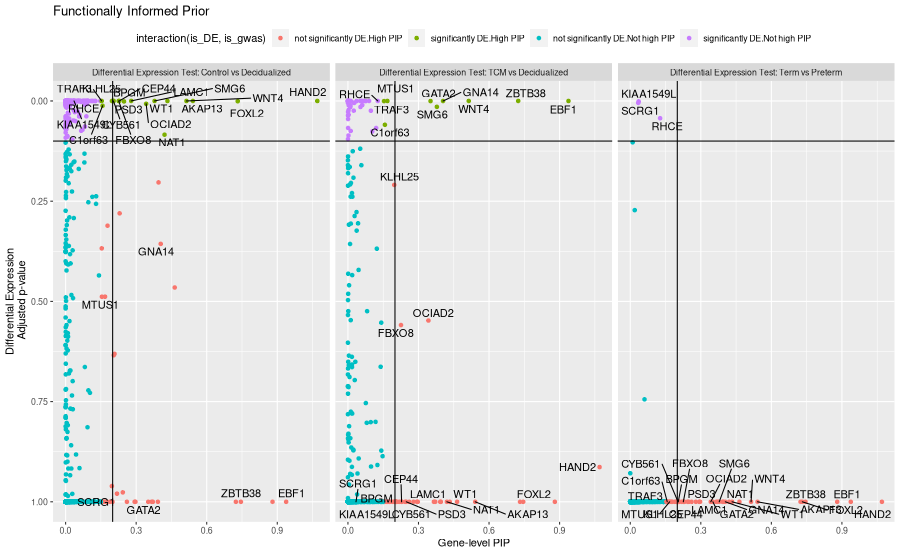
\includegraphics[width=\linewidth]{img/de-gwas-comp.png}
    \caption{Differential expression adjusted $p$-value for each of three differential expression tests: control vs decidualized, decidualized vs TCM-treated, and term vs preterm, along with the gene-level PIP for the corresponding gene for the 686 genes in the 33 genomic regions most likely to contain a gestational duration GWAS variant.  The vertical and horizontal lines indicated thresholds that were used to test for the enrichment of high PIP genes for differentially expressed genes. High PIP genes were significantly enriched for both differential control vs decidualized genes ($p=0.0264$), and for differential decidualized vs TCM-treated genes ($p=0.0344$), by fisher's exact test.}\label{fig:multiv_assoc}
    \end{subfigure}
\end{figure}




\section{Discussion}\label{sec:org53f1196}

 The lack of complete independence between these marks makes it difficult to delineate their individual effects but nonetheless highlights the importance of enhancers and of gene regulation in endometrial stromal cells in modulating the effects of GWAS variants on gestational duration. This is consistent with both the known tissue-specific roles of enhancers and the observation that over 90\% of GWAS loci reside outside of the coding portion of the genome and are enriched in regions of open chromatin and enhancers(12, 40). 

    Integrating transcriptional and chromatin annotations of gene regulation from MSCs and DSCs improved our ability to discover novel GWAS loci and identify likely causal SNPs and genes associated with gestational duration. We illustrate how our integrated platform identified a novel causal locus and candidate gene (HAND2) associated with gestational duration, as well as refined the annotation of loci that had been previously identified. Our data suggest that in endometrial stromal cells GATA2 is likely the target gene of enhancers harboring SNPs associated with gestational duration. This does not exclude the possibility that the nearest gene to the associated SNPs, EEFSEC, may be a target gene in other cell types.  

    Both of these examples highlight transcription factors that are essential for endometrial development or decidualization. The fact that neither GATA2 nor HAND2 were identified as potential candidate genes in previous GWASs of gestational duration or PTB supports our approach and the importance of using functional annotations from cell types relevant to pregnancy to fine map and identify candidate genes for the pregnancy-related traits. Overall, the integrated analyses performed in this study resulted in the identification of both novel GWAS loci and novel candidate genes for gestational duration, as well as maps of the regulatory architecture of these cells and their response to decidualization. 

    However, there are some limitations. Our results are based on only 3 individuals, which may not be enough to fully capture the regulatory landscape of endometrial stromal cells. In addition, the 3 individuals were African American and the GWAS results were obtained from Caucasians individuals and therefore, it is possible that the GWAS results do not match functional annotations in a different population, which could lead to erroneous conclusions. Another limitation is the fact that we focused on only one cell type, albeit one that plays a central role in pregnancy, and only one exposure (hormonal induction of decidualization) and only for 48 h. Different exposures could lead to different results. Future studies that include fetal cells from the placenta and uterine or cervical myometrial cells could reveal additional processes that contribute to gestational duration and PTB, such as those related to fetal signaling and the regulation of labor, respectively. Inclusion of additional exposures, such as trophoblast conditioned media(49), may further reveal processes that are pregnancy-specific. Second, to maximize power we focused on a GWAS of gestational duration and not PTB per se. While previous GWAS have shown that all PTB loci were among the gestational age loci(5), we realize that some of the loci that we identified could be related to normal variation in gestational duration and not specifically to PTB. Nonetheless, our findings contribute to our understanding of potential mechanisms underlying the timing of human gestation, about which we still know little. Lastly, although our ChIP-seq results revealed an association between GATA2 binding and decidualization, confirming the role of this transcription factor in decidual cell biology(50, 51), and studies in murines support its role in endometrial processes(34), we do not yet have direct evidence showing that perturbations in the expression of GATA2, or any of the other target genes identified, influence the timing of parturition in humans. Future studies will be needed to directly implicate the expression of these genes in gestational duration or PTB. Our study highlights the importance of generating functional annotations in pregnancy-relevant cell types to inform GWASs of pregnancy-associated conditions. Our results suggest that the expression of two transcription factors, GATA2 and HAND2, in endometrial stromal cells may regulate transcriptional programs that influence the timing of parturition in humans, which could lead to the identification of biomarkers of or therapeutic targets for PTB




% \subsubsection{A comment on distance to the nearest gene}


% ``Nearest gene'' is a an important benchmark when considering alternative methods for associating a variant with a gene\cite{fine2019benchmarker}.  In measuring the distance between a particular variant and surrounding genes, uncertainty may arise as as consequence of the ambiguity around the term ''gene''.



% Without attempting to define what a ge  to which gene is Without diverting iThere are several scenarios where the gene that is closest to a given variant depends on the definition of ``clo  distance from a variant to a gene can be calculated in One common approach for measuring the distance between variants to genes is to take the distance between        for evaluating the effectiveness of a snp-gene mapping distance to TSS is relevant for enhancer promoter looping conditioned on transcription initiation, what's the relevance of distance to TSS?
% Introns are worthy of special consideration, as they constitute approximately 25 percent of the human genome, and as they are, by definition, close to while distinct from the coding regions of the genome.    

% There are many possible mechanisms by which an intronic variant might act through a (protein-coding) gene to drive GWAS signal.
% Disrupting an enhancer is one such mechanism, but there are many additional mechanisms that involve altering transcription downstream of initiation.   (e.g APA, erroneous splice site, promoting RNA degradation, stalling elongation) and none of those really relate to distance to TSS.    For "early" introns/small genes the distance to TSS won't be much different from distance to nearest exon so it won't really matter, and for "late" exons in big genes the distance to the next downstream gene's TSS could be much closer to the variant.   Even if enhancers are very likely to target the nearest TSS (rather than nearest gene), you are more or less discounting all other causal mechanisms when you define "distance to gene" to be distance to TSS.
% 1:23 by "most of the mechanisms" I don't mean they're collectively more likely, I just mean there are many ways to disrupt a gene after transcription. lastly, the SNPs we're trying to assign to genes based on distance are going to (hopefully) be depleted for enhancers because of the HiC mapping step. Even if the non-enhancer mechanisms are relatively rare, they're more likely in our case.